\chapter{Ergebnisse} \label{evaluation}

In diesem Kapitel werden die Ergebnisse des Trainings und des Einsatzes der Objektdetektoren nach den in Kapitel \ref{eval} definierten Kriterien dargestellt. Es beinhaltet die Ergebnisse zur Präzision, zum Inferenzverhalten, zum Reaktionsvermögen und zum Trainingsverhalten der Detektoren.

\section{Präzision und Inferenzverhalten}

\subsection*{SSD}

Ursprünglich wurden 500 Epochen für das Training vorgesehen. Da allerdings beim Training schon nach knapp über hundert Epochen sich der Gradient der Kostenfunktion nur träge veränderte, wurde im Sinne des \textit{Early Stoppings} nach 121 Epochen das Training vorzeitig beendet, um \textit{Overfitting} zu vermeiden. Abbildung \ref{ssdloss} zeigt den Verlauf der Trainingsverlustkurve und der Testverlustkurve während des Kreuzvalidierungsverfahrens.

\begin{figure}[H]
	\begin{center}
		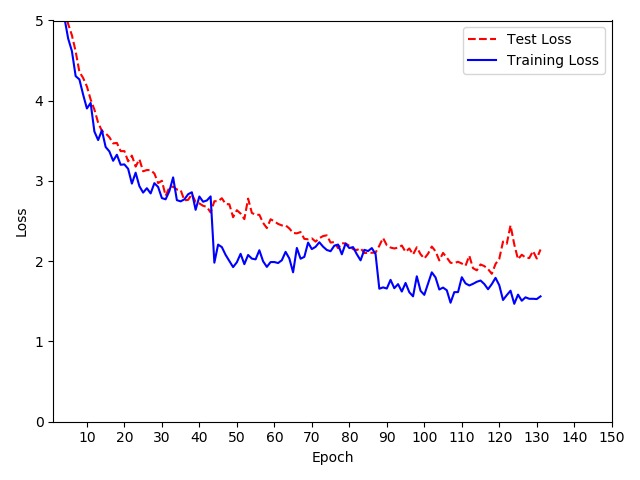
\includegraphics[width=8cm]{Bilder/ssdloss.jpeg} 
		\caption{Entwicklung der SSD Trainings- und Testverlustkurve während dem Training}
		\label{ssdloss}
	\end{center}
\end{figure}

Die Entscheidung zum \textit{Early Stopping} basiert auf dem Anstieg der Differenz zwischen Trainings- und Testverlustkurve ab Epoche 122, was auf \textit{Overfitting} schließen lässt. Zur Epoche davor war die Differenz der beiden Kurven am niedrigsten bei vergleichsweise geringem Verlust im Trainingsverfahren. Auffällig ist ebenfalls der große Abfall der Trainingsverlustkurve bei Epoche 45 und Epoche 89. Hier findet ein Wechsel im Kreuzvalidierungsverfahren statt. Die bessere Generalisierungsfähigkeit des Modells bei neuen Testdaten zeigt Ausschlag, indem die Klassifikationsergebnisse schlagartig besser werden und zu niedrigeren Kosten führen. Auch in Epoche 67 ist einer dieser Ausschläge zu sehen, der allerdings kleiner im Vergleich zu den anderen ausfällt. 

Zur Epoche 121 betrug das Ergebnis der Kostenfunktion 1.7. Es ergab eine \textit{mAP} von 83.1\%, leicht über den Referenzergebnissen von \textit{SSD} zu \textit{PascalVOC} (siehe Abbildung \ref{result}). Die Ergebnisse zu den einzelnen Klassen sind in folgender Tabelle dargestellt:

\begin{center}
	\begin{tabular}[H]{l|c}
		Klasse & mAP \\
		\hline
		Saskia Wasser Groß & 77.62\% \\
		Saskia Wasser Klein & 75.96\% \\
		Pepsi Cola Groß & 94.94\% \\
		Pepsi Cola Klein & 86.38\% \\
		ISO & 86.37\% \\
		ACE & 85.43\% \\
		Stenger Johannisbeerschorle & 69.47\% \\
		Stenger Apfelsaftschorle & 82.48 \% \\
		Vitamalz Malzbier & 76.24\%
	\end{tabular}
	\captionof{table}{Validierungsergebnisse SSD}
	\label{table:ssdresults}
\end{center}

Wird nun das trainierte Modell auf echte Daten angewendet, so fällt auf, dass manche Objekte doppelt detektiert werden. Um dieses Problem zu lösen, gibt es zwei Möglichkeiten. 

Als erstes kann bei der Detektion der minimale \textit{confidence score} angegeben werden, ab wann eine Detektion offiziell als solche wahrgenommen wird. Hier liegt die Herausforderung darin, einen optimalen Wert zu finden, sodass verdeckte Objekte noch als solche erkannt werden, aber doppelt erkannte Objekte nicht mehr auftreten. Der \textit{confidence score} wurde nach mehrmaligem Iterieren auf 0.7 festgelegt.

Die zweite Möglichkeit besteht darin, die maximale Überlappung zweier Bounding Boxen festzulegen. Somit werden doppelte Bounding Boxen, die sich flächenmäßig über einem gewissen Grenzwert überlappen, auf eine Bounding Box reduziert. Er stellte ich sich Parameter von 0.45 als geeignet heraus. Außerdem wurden Inkonsistenzen im Detektionsverhalten festgestellt.

\begin{figure}[H]
	\subfigure[Verdecktes Objekt I]{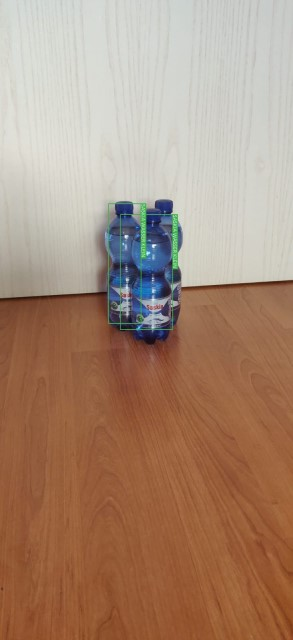
\includegraphics[width=0.20\textwidth]{Bilder/verdeckt.jpeg}}\hfill
	\subfigure[Verdecktes Objekt II]{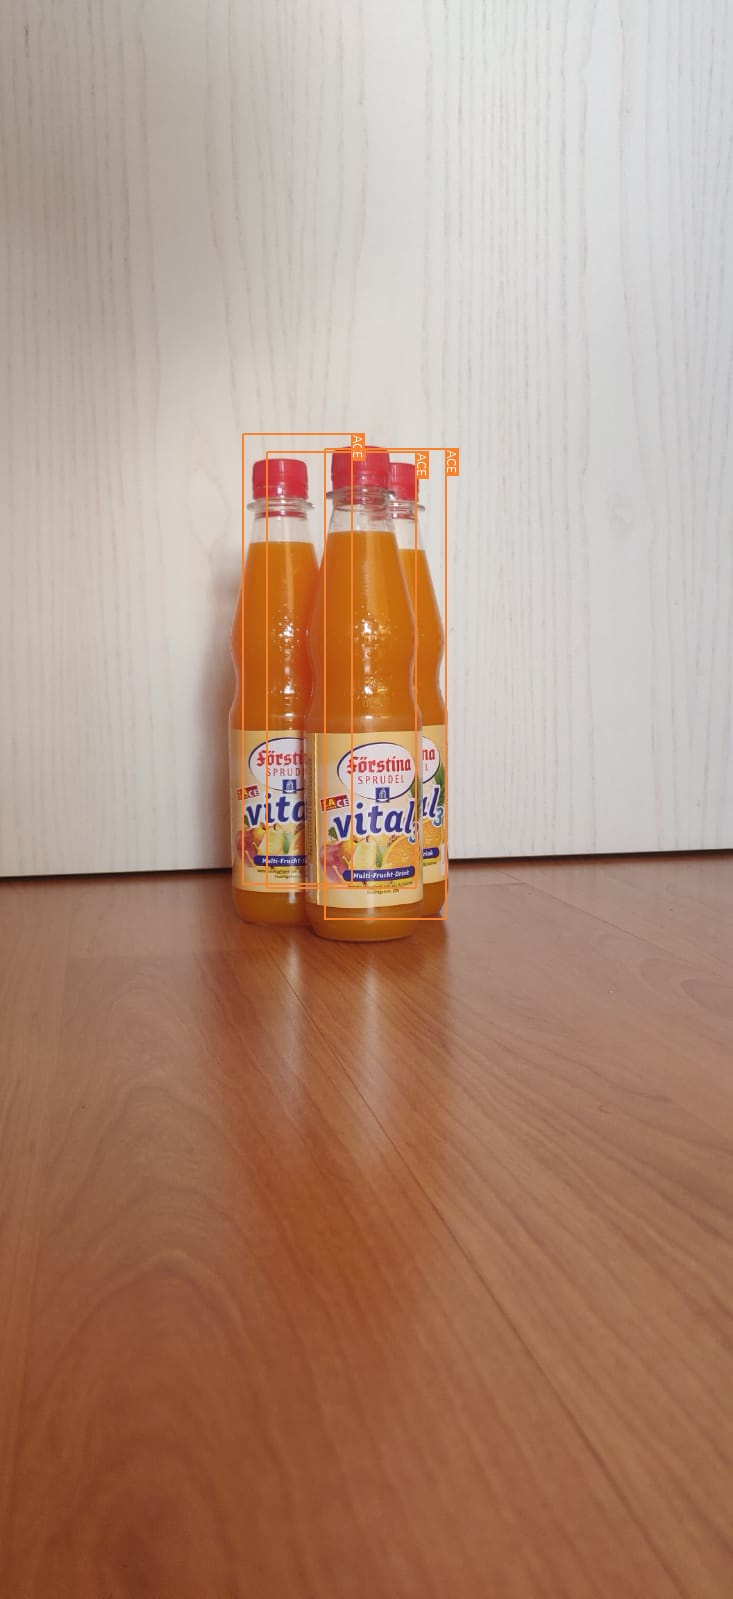
\includegraphics[width=0.20\textwidth]{Bilder/verdeckt2.jpeg}}\hfill
	\subfigure[Extreme Blicklagen I]{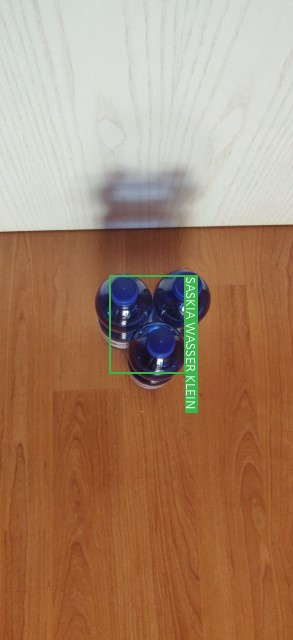
\includegraphics[width=0.20\textwidth]{Bilder/winkel.jpeg}}\hfill
	\subfigure[Extremen Blicklagen II]{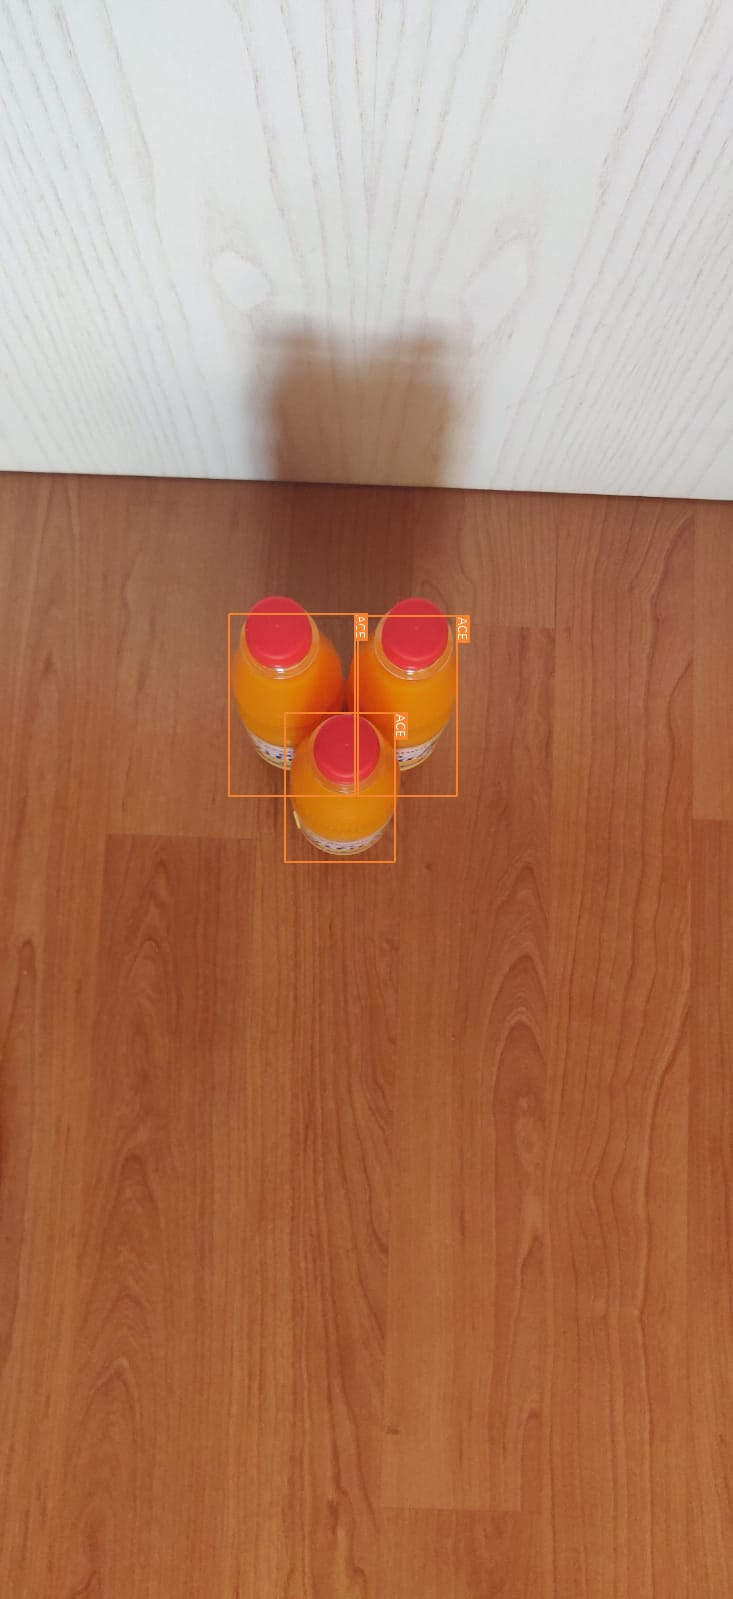
\includegraphics[width=0.20\textwidth]{Bilder/winkel2.jpeg}}
	\caption{Detektionsverhalten von SSD bei extremen Blicklagen}
	\label{lagen}
\end{figure}

So sind von anderen Objekten verdeckte Objekte nur schwer zu erkennen. So wird beispielsweise in Abbildung \ref{lagen} (a) das rechte hintere Objekt selbst bei einem sehr niedrigen \textit{confidence score} Schwellwert nicht erkannt. In Abbildung \ref{lagen} (b) hingegen ist eine Detektion ab einem \textit{confidence score} von 0.53 möglich, was allerdings wieder weitere ungenaue und ungewünschte Detektionen verursacht. Ähnliche Probleme ergeben sich für die Detektion von Objekte aus extremen Blicklagen. In Abbildung \ref{lagen} (c) werden die Objekte beispielsweise erst ab einem \textit{confidence score} von 0.54 erkannt, allerdings nicht als drei einzelne Objekte, sondern als ein großes Gesamtobjekt. Dies gilt allerdings nicht für alle Klassen. Bei Anwendung dieses Problemfalls auf eine andere Klasse ergeben sich bei vergleichbarem \textit{confidence score} von 0.56 sehenswertere Ergebnisse (siehe Abbildung \ref{lagen} (d)). 

Die zwei genannten Problemfälle wurden im Datensatz zwar zu 12.5\% abgedeckt, scheinen allerdings nur wenig Auswirkung auf besseres Detektionsverhalten für solche Fälle geliefert zu haben. Es lässt sich auch keine Aussage darüber treffen, ob eine Erweiterung des Datensatzes mit weiteren solchen Extremfällen eine Abhilfe für dieses Problem hätte liefern können. 

\begin{figure}[H]
	\subfigure[1 Meter]{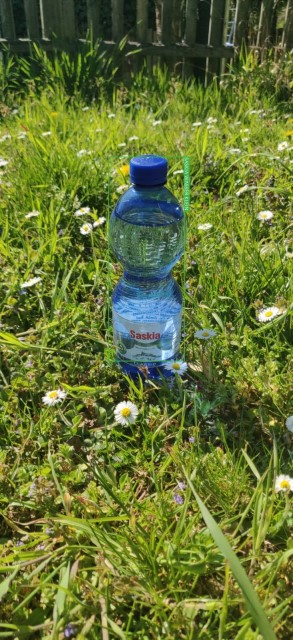
\includegraphics[width=0.30\textwidth]{Bilder/einmeter.jpeg}}\hfill
	\subfigure[2 Meter]{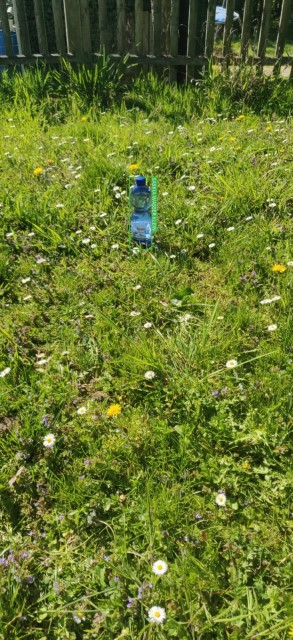
\includegraphics[width=0.30\textwidth]{Bilder/zweimeter.jpeg}}\hfill
	\subfigure[3 Meter]{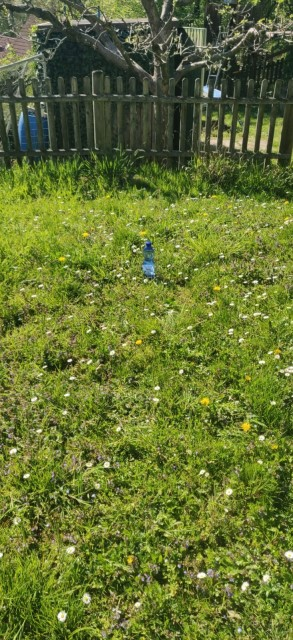
\includegraphics[width=0.30\textwidth]{Bilder/dreimeter.jpeg}}\hfill
	\caption{Detektionsverhalten von SSD bei unterschiedlichen Entfernungen}
	\label{entfernung}
\end{figure}

Auch die Entfernung zum zu detektierenden Objekt besitzt eine Auswirkung auf das Detektionsverhalten. In Abbildung \ref{entfernung} wird gezeigt, dass ab einer Entfernung von drei Metern eine zuverlässige Detektion nicht mehr möglich ist. In diesem Beispiel ist erst ab einer niedrigeren \textit{confidence score} Grenze von 0.31 eine Detektion des Objekts wieder erfolgt, bei anderen Beispielen sogar erst ab einem Wert von 0.09.

\begin{figure}[H]
	\subfigure[überbeleuchtet I]{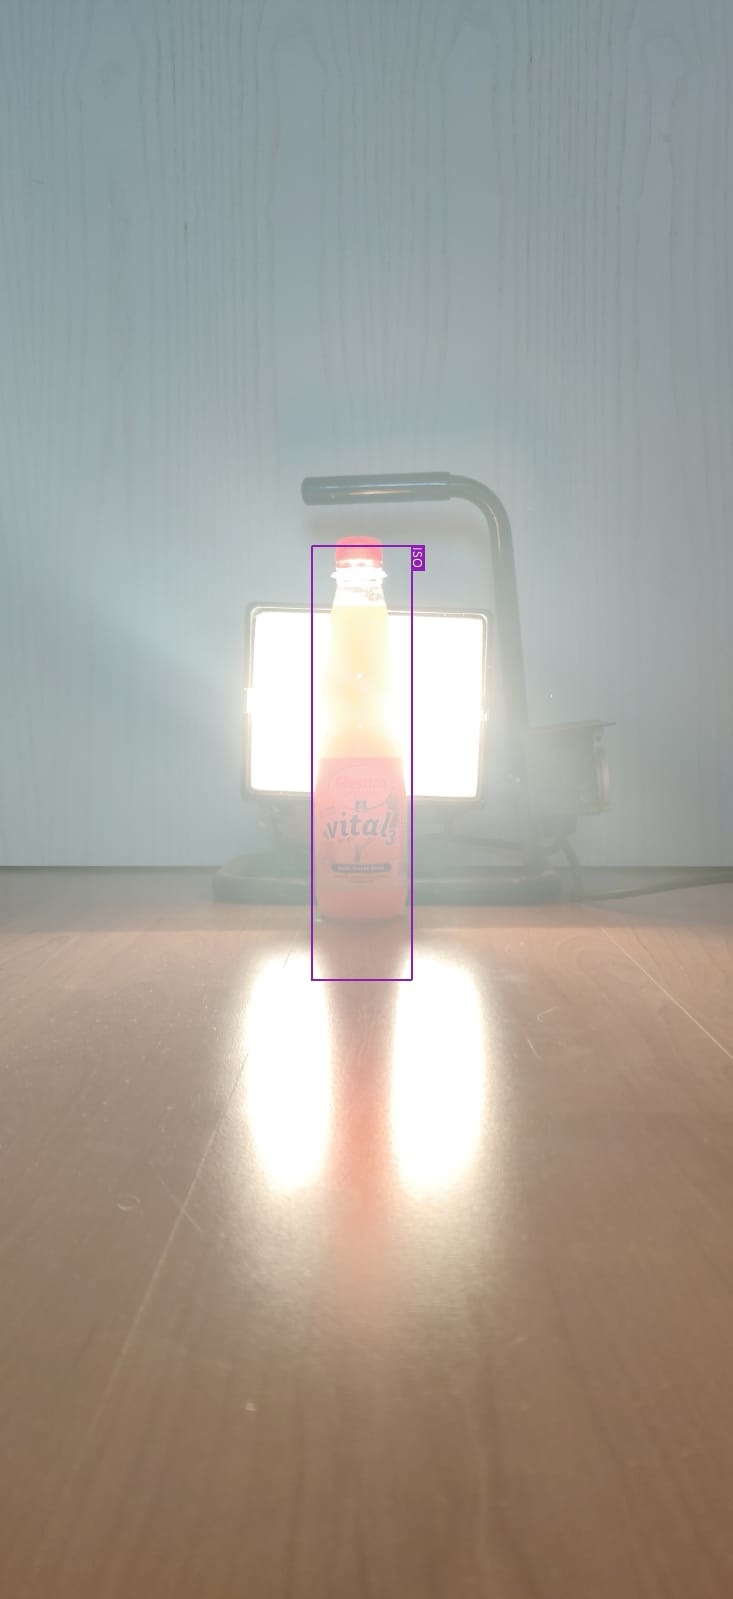
\includegraphics[width=0.20\textwidth]{Bilder/ueberbeleuchtet2.jpeg}}\hfill
	\subfigure[überbeleuchtet II]{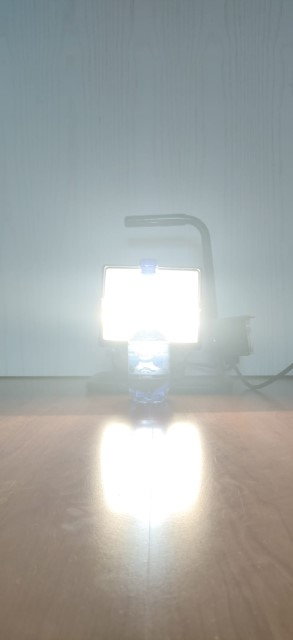
\includegraphics[width=0.20\textwidth]{Bilder/ueberbeleuchtet.jpeg}}\hfill
	\subfigure[normal]{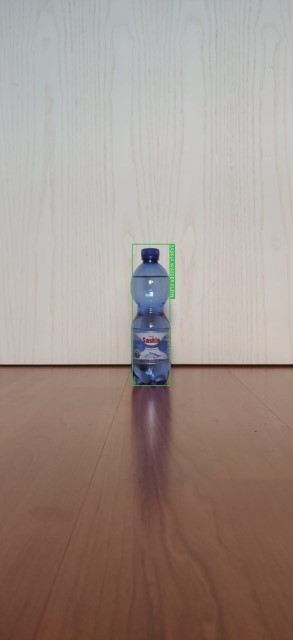
\includegraphics[width=0.20\textwidth]{Bilder/normalbeleuchtet.jpeg}}\hfill
	\subfigure[unterbeleuchtet]{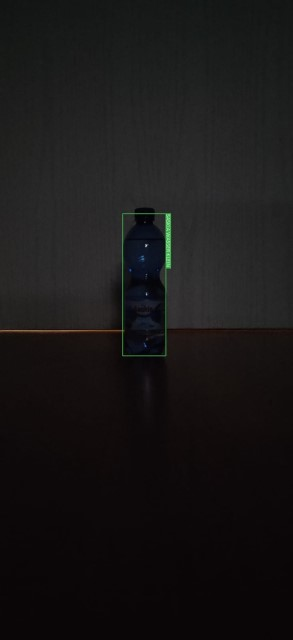
\includegraphics[width=0.20\textwidth]{Bilder/unterbeleuchtet.jpeg}}\hfill
	\caption{Detektionsverhalten von SSD bei unterschiedlichen Beleuchtungsverhältnissen}
	\label{sicht}
\end{figure}

Des Weiteren haben unterschiedliche Beleuchtungsgrade eine Auswirkung auf das Detektionsverhalten. In Abbildung \ref{sicht} wird unterschieden zwischen dem Detektionsverhalten bei überbeleuchteten, normalen und unterbeleuchteten Sichtverhältnissen. Überbeleuchtete Umgebungsverhältnisse erschweren die Objektdetektion. Zum einen können bestimmte Objekte gar nicht mehr erkannt werden (siehe Abbildung \ref{sicht} (b)) oder die dadurch verursachte Lichtabsorption und anschließende Emission durch die zu detektierenden Objekte führt zu einer Falschdetektion. In Abbildung \ref{sicht} (a) wird so beispielsweise mit einem \textit{confidence score} von 0.91 das Objekt der Klasse \textit{ACE} falsch als \textit{ISO} klassifiziert.

Alle Detektionen reagierten allerdings invariant gegenüber unterschiedlichen Hintergründen oder Bildauflösungen.

\subsection*{YOLO}

Um eine möglichst gute Aussage über den Vergleich der beiden Objektdetektoren treffen zu können, kommt bei \textit{YOLO} der exakt gleiche Trainings- und Testdatensatz wie beim \textit{SSD} zum Einsatz. Das Training von \textit{YOLO} ergab eine \textit{mAP} von 80.36\%. Abbildung \ref{yolo_result} zeigt die Verbesserung des Modells während dem Trainingsprozess. 

\begin{figure}[H]
	\begin{center}
		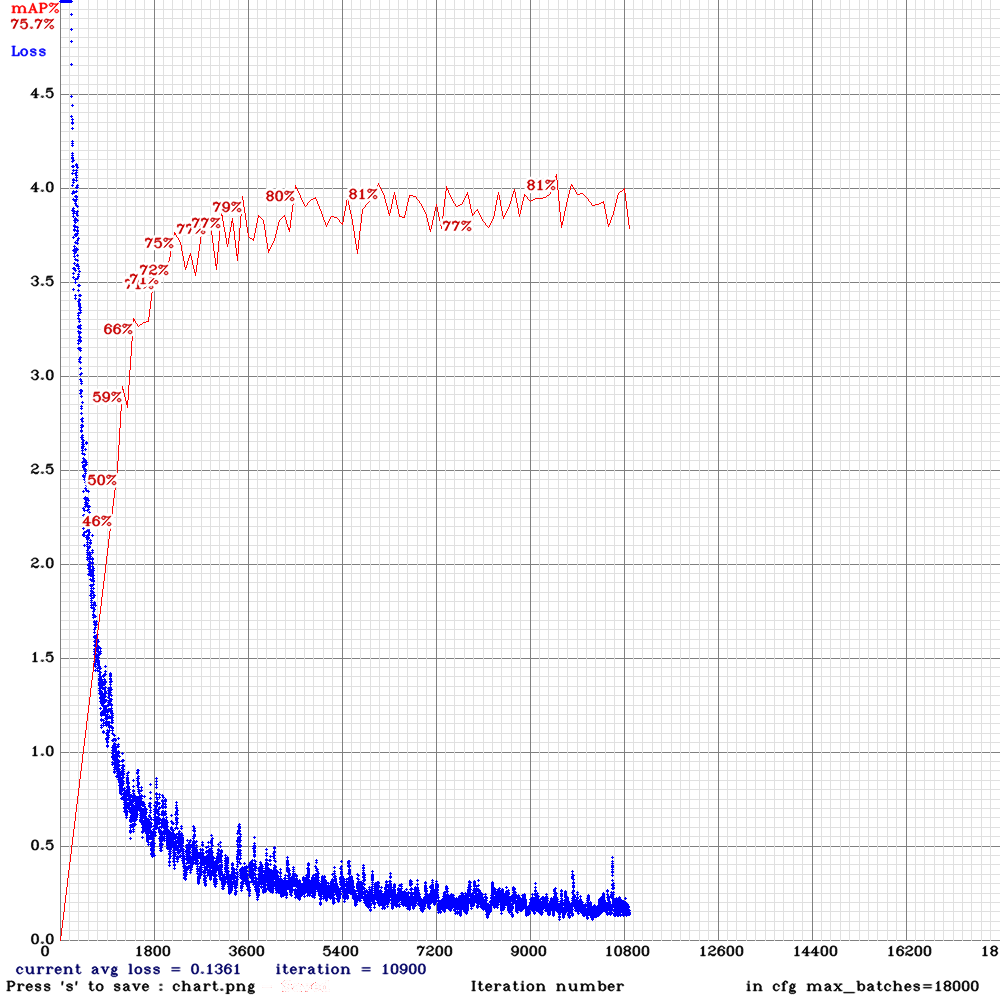
\includegraphics[width=8cm]{Bilder/yolo_result.png} 
		\caption{Entwicklung der YOLO Testverlustkurve und der \textit{mAP} während dem Training}
		\label{yolo_result}
	\end{center}
\end{figure}

Wie beim \textit{SSD} erreicht das Modell nach bereits etwa 4500 Batches eine \textit{mAP} von 80\%. Da sich das Modell ab diesem Zeitpunkt nicht mehr maßgeblich verbessert hat, wurde das Training vor Erreichung der durch die Dokumentation nahegelegte maximale Anzahl an Batches abgebrochen. Das frühe Erreichen eines sehr guten Ergebnis kann darauf zurückgeführt werden, dass es sich bei den gelabelten Klassen um Objekte des gleichen Typs handelt und das Modell dementsprechend leichter trainiert werden kann. 

Der \textit{confidence score} liegt standardmäßig bei 0.25. Nach mehreren Durchläufen stellt sich heraus, dass dieser Wert nicht verändert werden sollte. Ein zu geringer Wert sorgt zwar dafür, dass möglicherweise mehr Objekte erkannt werden, allerdings steigt damit auch die Rate an falsch oder doppelt erkannter Objekte. Ein Parameter für die Obergrenze der Überlappung zweier Bounding Boxen existiert nicht.

Tabelle \ref{table:yoloresults} zeigt die \textit{mAP} für jede Klasse.

\begin{center}
	\begin{tabular}[H]{l|c|c}
		Klasse & mAP & Differenz zu SSD\\
		\hline
		Saskia Wasser Groß & 76.69\% & (-0.93\%) \\
		Saskia Wasser Klein & 80.63\% & (+4.67\%) \\
		Pepsi Cola Groß & 73.14\% & (-21.8\%) \\
		Pepsi Cola Klein & 75.24\% & (-11.14\%) \\
		ISO & 90.28\% & (+3.91\%) \\
		ACE & 86.69\% & (+1.26\%) \\
		Stenger Johannisbeerschorle & 72.50\% & (+3.03\%) \\
		Stenger Apfelsaftschorle & 78.05\% & (-4.43\%) \\
		Vitamalz Malzbier & 81.94\% & (+5.7\%)
	\end{tabular}
	\captionof{table}{Validierungsergebnisse YOLO im Vergleich zu SSD}
	\label{table:yoloresults}
\end{center}

Auch bei \textit{YOLO} können verdeckte Objekte nur schwer erkannt werden. Ein Unterschied zu \textit{SSD} zeigt sich bei der Ansicht von oben:

\begin{figure}[H]
	\centering
	\subfigure[verdeckt]{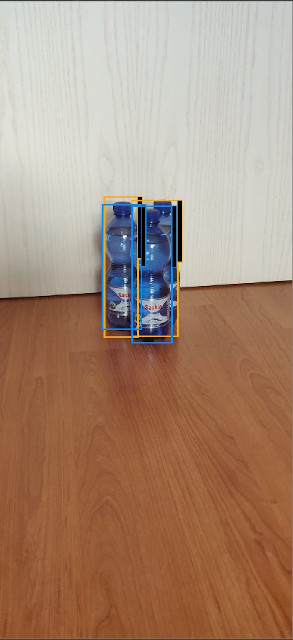
\includegraphics[width=0.30\textwidth]{Bilder/yolo_verdeckt.jpg}}
	\hspace{2cm}
	\subfigure[winkel]{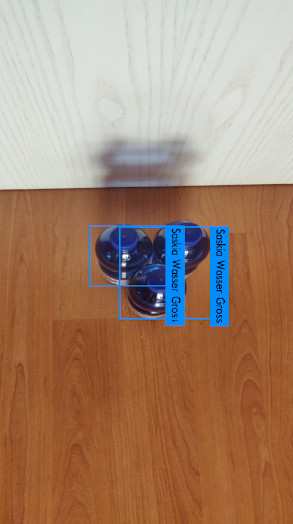
\includegraphics[width=0.30\textwidth]{Bilder/yolo_winkel.jpg}}
	\caption{Detektionsverhalten von YOLO bei extremen Blicklagen}
	\label{lagen_yolo}
\end{figure}

Hier werden zwei von drei Flaschen erkannt, die allerdings der falschen Klasse (\textit{Saskia Wasser Groß} statt \textit{Saskia Wasser Klein}) zugeordnet werden und eine der zwei Bounding Boxes zwei Flaschen umschließt.

\begin{figure}[H]
	\subfigure[1 Meter]{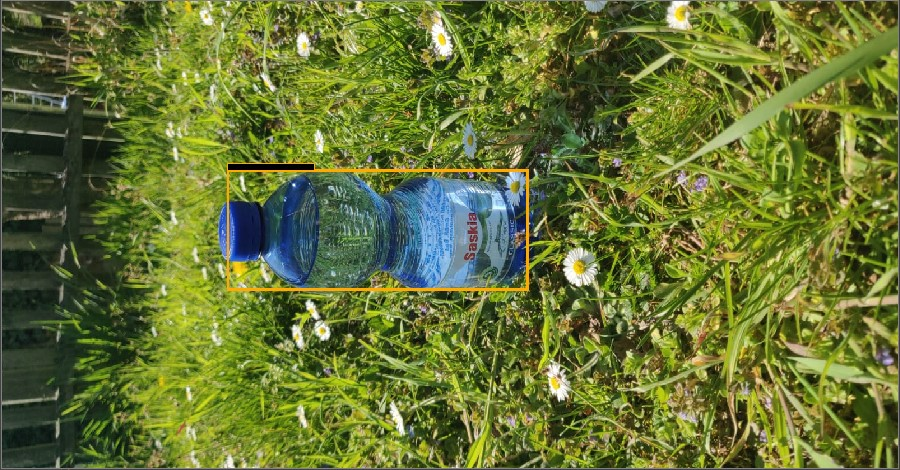
\includegraphics[width=0.30\textwidth]{Bilder/yolo_entfernung1.jpg}}\hfill
	\subfigure[2 Meter]{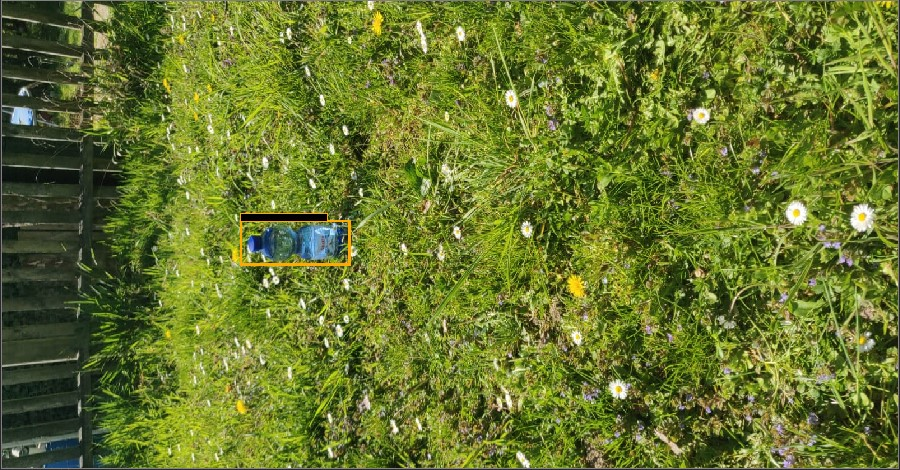
\includegraphics[width=0.30\textwidth]{Bilder/yolo_entfernung2.jpg}}\hfill
	\subfigure[3 Meter]{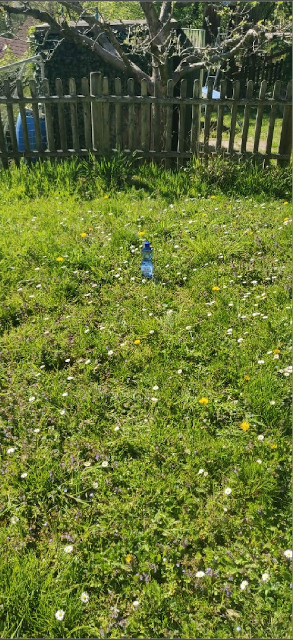
\includegraphics[width=0.30\textwidth]{Bilder/yolo_entfernung3.jpg}}\hfill
	\caption{Detektionsverhalten von YOLO bei unterschiedlichen Entfernungen}
	\label{entfernung_yolo}
\end{figure}

Wie bei \textit{SSD} erfolgt nach bereits drei Metern Entfernung keine Detektion mehr (siehe Abbildung \ref{entfernung_yolo}). Der \textit{confidence score} für die korrekt erkannte Bounding Box liegt bei nur 2\%.
 
\begin{figure}[H]
 	\subfigure[überbeleuchtet]{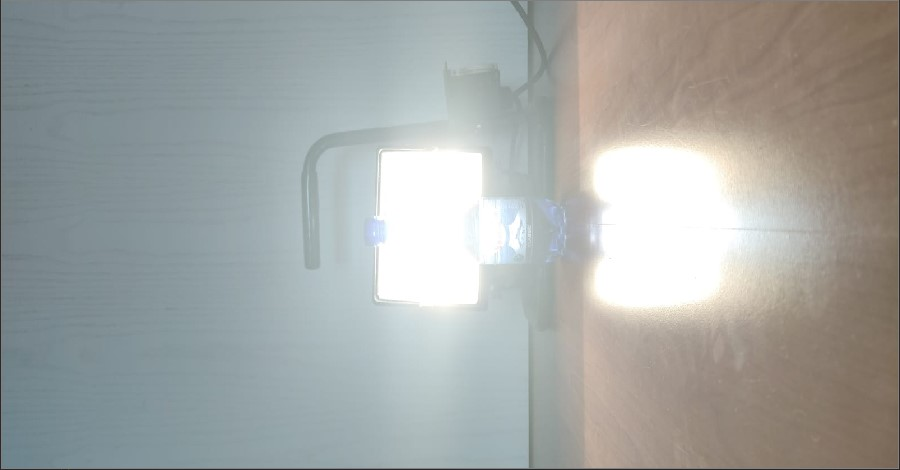
\includegraphics[width=0.30\textwidth]{Bilder/yolo_beleuchtung2.jpg}}\hfill
 	\subfigure[normal]{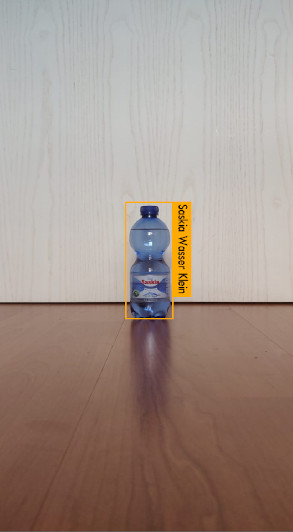
\includegraphics[width=0.30\textwidth]{Bilder/yolo_beleuchtung1.jpg}}\hfill
 	\subfigure[unterbeleuchtet]{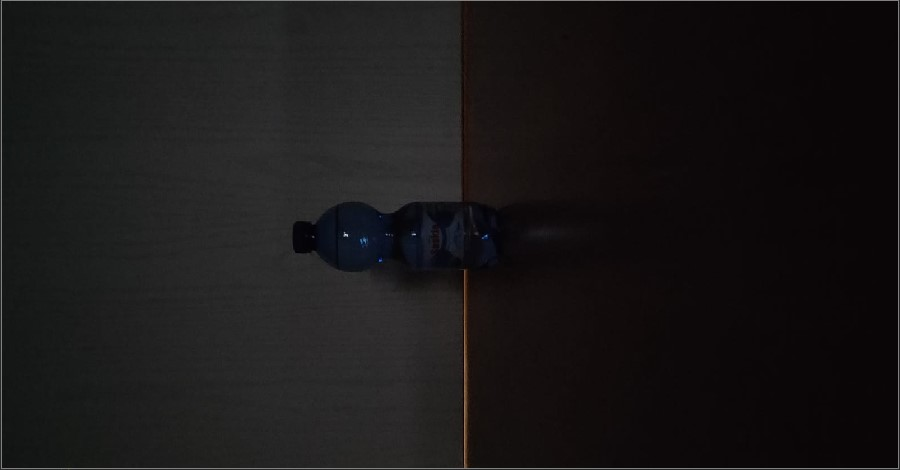
\includegraphics[width=0.30\textwidth]{Bilder/yolo_beleuchtung3.jpg}}\hfill
 	\caption{Detektionsverhalten von YOLO bei unterschiedlichen Beleuchtungsverhältnissen}
 	\label{sicht_yolo}
\end{figure}

Beim Testen der verschiedenen Beleuchtungsverhältnisse fällt auf, dass im Gegensatz zum \textit{SSD} die Flasche in der unterbelichteten Umgebung nicht erkannt wird beziehungsweise mit einem \textit{confidence score} von nur 6\%. 

Gleich zu \textit{SSD} reagiert \textit{YOLO} auch invariant gegenüber unterschiedlichen Hintergründen oder Bildauflösungen.
 
\section{Reaktionsvermögen}

Bei der Inferenz fällt allerdings entgegen der Erwartungen auf, dass die Inferenz überdurchschnittlich langsam verläuft. Das Problem lässt sich auf die synchrone Arbeitsweise der bisherigen Detektionsalgorithmen zurück führen, bei dem erst ein neuer Frame des Videostreams angefragt wird, sobald das aktuelle Bild durch die Vorverarbeitung gelaufen ist und durch das Modell inferiert wurde. 

Um dem entgegen zu wirken, wurde ein Bufferkonzept in einem parallelem Thread realisiert, der einzelne Frames zeitgleich zur Inferenz anfragt und zwischenspeichert. Ist der Buffer voll, so werden nach dem \textit{First In First Out} Verfahren die älteren Frames verworfen. Dadurch konnte die FPS Anzahl von \textit{SSD} von maximal 18 auf die vollen 30 und bei \textit{YOLO} von 20 auf 28 gesteigert werden. Dadurch sollten sämtliche Änderungen in der Umgebung rechtzeitig vom Objektdetektor erkannt werden. 

Ein weiteres Problem beschreibt die initiale Latenz zwischen der Inferenz und der Bildaufnahme. Die Inferenz kann erst gestartet werden, sobald die Gewichtungen des Modells initialisiert und geladen wurden. Bei \textit{YOLO} benötigt die Initialisierung etwa drei Sekunden, bei \textit{SSD} vier Sekunden. Das lässt sich umgehen, indem entweder der Thread zur Bildaufnahme verzögern gestartet wird oder dessen Buffer kleiner gewählt wird.

\section{Trainingsverhalten}

\begin{center}
	\begin{tabular}[H]{l|c|c|c|c}
		Detektor & Hardware & Batchgröße & Dauer Epoche & Dauer Insgesamt \\
		\hline
		SSD & GTX 1080 & 16 & 9 Min. & 16.5 Std. \\
		YOLO & RTX 2060 & 64 & 1.5 Min. & 8 Std.
	\end{tabular}
	\captionof{table}{Trainingsverhalten von SSD und YOLO}
	\label{table:duration}
\end{center}

Tabelle \ref{table:duration} zeigt die Ergebnisse des Trainingsverhaltens von \textit{SSD} und \textit{YOLO}. Pro Epoche wurden 998 Bilder durchlaufen. Die Dauer der beiden Trainingsdurchläufe lässt sich allerdings nur schwer vergleichen. Zum einen wird für das Training von \textit{YOLO} eine andere GPU verwendet, deren Tensor Kerne den Trainingsprozess merklich beschleunigen. Zum anderen werden die beiden Objektdetektoren in zwei verschiedenen Frameworks implementiert, wodurch ein anderes Trainingsverhalten von Grund auf gegeben ist und Unterschiede in der Performance auftreten können. Auch die Batchgröße wurde unterschiedlich gewählt, was sich auf die Häufigkeit des Gradientenabstiegs auswirkt. Bei beiden Verfahren kann das Training durch die Ablage von sogenannten Modell-Checkpoints zu einem späteren Zeitpunkt fortgeführt werden. Das ist vor allem dann von Vorteil, wenn nachträglich Parameter oder Trainingsdaten angepasst werden und kein kompletter Neustart des Trainings erforderlich ist.
